\Chapter{
    ``For you are dust, and to dust shall you return.''
\\[5pt]
\rightline{{\rm --- The book of genesis 3:19}}
}{Background}
Aeolian dust is one the most abundant aerosol species in the atmosphere constituting the majority of the total atmospheric  aerosol mass. The main source regions of aeolian dust are regions such as the Sahara desert, the Middle East and desert regions in north west China. Once the dust is entrained into the atmosphere it can be transported over wast distances \parencite{yumimoto_elevated_2009}. While in the atmosphere the dust directly impacts earth’s radiative balance through scattering short wave radiation from the sun and absorbing long wave radiation. Dust also indirectly impacts climate by acting as cloud condensation nuclei (CCN) and ice nuclei (IN) affecting the cloud droplet number concentrations, which in turn alters the cloud optical properties and life time \parencite{lohmann2006sensitivity}. The dust will eventually settle and depending where the dust is deposited it can have a significant impact on the biogeochemistry e.g. acting as an important source of nutrients in the ocean \parencite{jickells_dust_biogeo_2015}. Yet current climate models struggles with reproducing many of  the effects has on climate dust, due to their inability to accurately simulate the important dust processes such as dust emissions, transport and deposition. 

In the first part of this chapter \Cref{sec:dust_modelling} will give an overview of the existing approaches for dust modelling. Outlining the physical that processes included in current dust models and what the main uncertainties are. Then the second part will focus on East Asian dust specifically and describe the characteristics of the main source, the meteorological conditions that responsible for producing dust events.     

%A cloud with a high droplet number concentration of a given cloud water content would be more optically thick, this is known as the aerosol cloud albedo effect. Secondly the            

%  \parencite{yumimoto_elevated_2009}    has been observed in   the largest in therms of mass   
% Dust is present almost every where 
% Dust can several associations depending on the context,  when talking about atmospheric dust one usually ref   Dust is an essential ingredient of our earth system.   

% P Aeolian dust is a fundamental component in the climate system. Large range of scales motion influences the emission 
% ,transport and deposition of aeolian dust from turbulent wind gust at the surface to large scale atmospheric circulation 
% patterns. The aim of this chapter is to the provide the necessary background for understanding the emission, deposition 
% and transport of East Asian aeolian dust. The first part of this chapter will focus on explaining the physics of dust 
% emissions, what are different processes and how do we model dust emissions, where are the major dust source regions in 
% East Asia and which kind of meteorological conditions favours dust emission. The second part will go into the transport 
% of aeolian dust, the role large scale circulation have on dust transport from East Asian desert. \todo{NEED to give 
% proper references to the different section}. The last part will look at the how mineral dust is deposited, how was the 
% Loess Plateau formed and how the Loess deposit can be an a window into understanding past climate.

\section{About dust modelling}\label{sec:dust_modelling}

\subsection{Dust emissions}\label{sec:dust_emission_modelling}
The first step of any dust model is to estimate the emission strength. Wind erosion is the consequence of a tug between the aerodynamic forces that tend to remove dust particles from the soil and forces that tend to fix the particles to ground such as gravity and inter-particle forces. The aerodynamic forces are normally quantified by the friction velocity $u^*$, which describe the amount of momentum transferred from the air to the surface. Then moment at which the aerodynamic forces exceed the forces counteracting wind erosion is described by the threshold friction velocity $u^*_t$. The balance between the $u^*$ and $u^*_t$ is sensitive to several environmental factors such as, weather (e.g. wind, precipitation and temperature), the soil composition, the soil moisture content, soil particle size distribution, vegetation converge and topography. All these factors vary significantly both spatially and temporally making accurately simulating dust emissions challenging to say the least.       
%This tug is quantified by a threshold friction velocity $u^*$  This involve determining the which regions are susceptible to wind erosion.  Almost all the processes related to wind erosion depend on the particle size. 

Many of the environmental factors have been accounted for based on empirical relations derived from several wind tunnel experiments and field measurement campaigns conducted during the last 50 years. In recent years observations from earth observing satellites such as the MODIS satellites have become increasingly important. This allowed for global monitoring of dust storm and to derived necessary land-surface and atmospheric parameters for dust modelling.    

There are two ways that dust is entrained into the atmosphere, either directly through aerodynamically entrainment or through sandblasting by saltating dust particles. Whether a dust particle is entrained through sand blasting or aerodynamic entrainment depends on the size of the dust particle. For a dust particle resting in the soil bed there are four forces acting on the dust particle. The forces promoting entrainment are aerodynamic lift ($F_l$) and aerodynamic drag $(F_d)$ and the opposing forces are the inter-particle forces $F_{ip}$ and the gravitational force $F_g$. For a dust particle to be aerodynamically entrained, $F_l$ and $F_d$ have to exceed $F_{ip}$ and $F_g$. Friction velocity is commonly used to describe to the flux of momentum from the atmosphere to surface and is a crucial parameter when doing dust modelling. The inter-particle forces dominate for small dust particles  (< $50\mu m $) and therefore a have too large threshold friction velocity in order to be directly entrained in the atmosphere by the winds \parencite{kok2012physics}. 

\subsection{Dust transport and depostion modelling}
\begin{figure}[htbp]
  \centering
  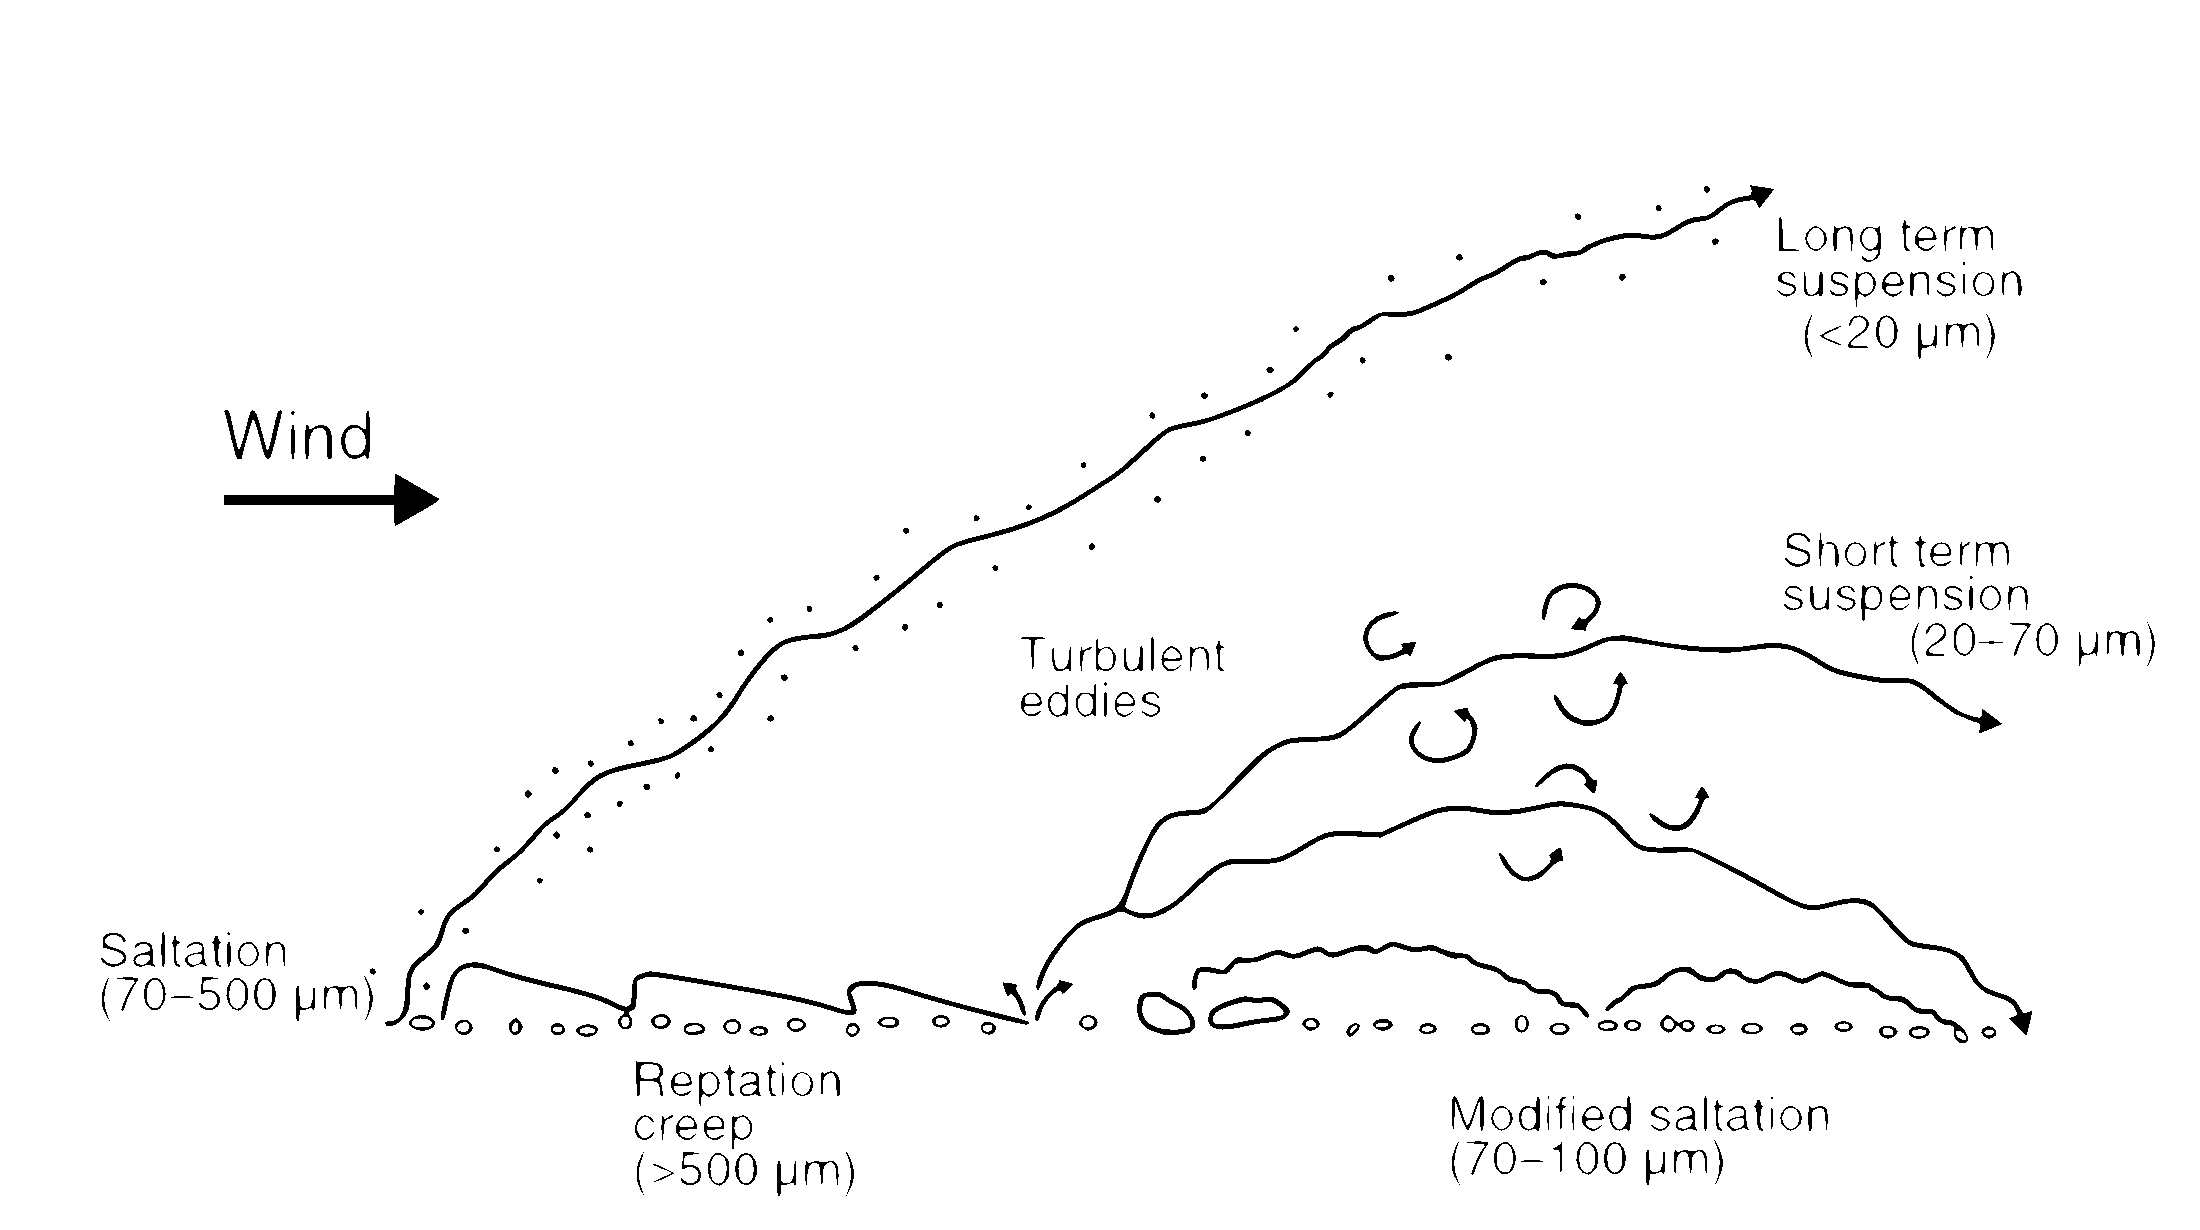
\includegraphics[width = \textwidth]{texfiles/figs/aeolian_transport_Parsons_Abrahams.pdf}
  \caption{Different regimes of aeolian transport \parencite{nickling2009aeolian}}
\end{figure}


Rather fine dust particles are ejected into atmosphere by larger dust particles splashing into the soil bed. Because the large particles have a  lower threshold friction velocity. \Cref{fig:treshold_friction_velocity_ps} shows the friction velocity required for a dust particle to be aerodynamically lifted as a function of equivalent particle diameter, and we see that the minimum in threshold friction velocity occur between \SI{75}{\micro\metre} - \SI{100}{\micro\metre}.

\section{Lagrangian Models}
An advantage with Lagrangian models is that they essentially do not exhibit numerical diffusion, except for errors related to interpolating the meteorological input data to the particle positions, in contrast to Eulerian models which often suffer from numerical diffusion \parencite{cassiani_offline_2016}. \textcite{cassiani_offline_2016} evaluated the offline FLEXPART-NorESM against the online tracer solver within NorESM and showed that the horizontal diffusion was around 10 times stronger for the online NorESM solver compared to the offline FLEXPART-NorESM. 

An interesting possibility of LPDM is that they can be run can either be run forward or backwards in time, by simply switching the sign of the advection. Forward simulation, are a natural choice for studying the dispersion of tracers from known sources, for example the dispersion of nuclear fallout where you have one point source but an unknown number of receptors. While a forward simulation indicate where an atmospheric tracer will go, a backward simulation indicate where the tracer came from. Therefore backward simulations are useful for interpreting measurements of atmospheric trace substances and to establish relationships between the sources and their receptors.  


\section{East Asian Dust}

\subsection{Atmospheric circulation in East Asia}
The most prominent feature of the atmospheric circulation in the East Asian region is the monsoon system. A monsoon wind system is one that seasonally changes direction, blowing from one direction in the summer and in the opposite direction in the winter.  The primary driver of the East Asian monsoon system is the temperature contrast between the land and ocean. During the winter months the land is generally colder than the ocean where the main heating source is located over the equatorial western pacific. The convection associated with the heating drives a large scale meridional overturning circulation where the airmasses rises over the ocean and then subsides over the Sebrian region. Creating a persistent high pressure system over Sebria during the winter. This circulation is the East Asian Winter Monsoon (EAWM). During the East Asian Summer Monsoon (EASM) the situation is reversed. In the summer the land is much warmer than the ocean, the heating on land drives strong convection which creates a persistent low pressure at the surface. The low pressure drags moist air from the ocean inland. Upon reaching the Tibetan Plateau the moist air is lifted and consequently cooled which causes the water vapor to condense resulting in intense precipitation. 

In following section will describe the EAWM and EASM circulation and how they are influenced by ...   

\subsection{East Asian Winter Monsoon}
The EAWM dominates the climate in East Asia during winter months, December, January, February, and is closely related to the cold core of the Siberian High.  

\section{Physics of windblown dust}
it has been known that there are three major motions of wind‐blown sand particles, i.e., creep, saltation, and suspension

Except for dust storms in which the suspension motion is dominant, saltation plays a key role in the wind erosion process
\subsection{Deserts regions in East Asia}
The main desert regions in east Asia is the Gobi Desert, Taklamakan desert, Badain Jaran Desert, \todo{Need map} and the Mu Us Desert. The Taklamakan desert is located in the tarim basin is the second largest sand desert in the world. The desert is surrounded by tall mountain ranges on both sides which can mechanically lift dust veils into the upper tropshere \parencite{yumimoto_elevated_2009}.   There are difference in soil composition between the different deserts. Gobi Desert is a primarialy stone desert, compared to Badain Jaran and Taklamakan which both sandy desert. The Badain Jaran desert has the tallest sanddunes in the planet. 





\subsection{Source receptor relationships within the framework Lagrangian particle dispersion models}

The problem with using ordinary Lagrangian trajectory model to calculate trajectories is that measurements 
often represent large volumes of air and not infinitesimally small air parcels (from now on referred to as 
particles). Therefore a single particle trajectory is usually not representative of the trajectory of the 
whole volume element. This is to due deformation and stretching of the fluid elements. This deformation 
happens for example if the flow has to pass an obstacle eg. a mountain range, the initially compact fluid 
elements would be torn apart and distributed over large areas. Moreover the separation and distortion of the
volume element would be even more effective in the presence of strong vertical wind shear causing fluid 
elements to travel in opposite direction. Which means that two particles that are at the beginning close to 
each other would given enough time would eventually be separated by large distances. Another issue with the 
single particle approach is that the turbulence of the atmosphere would increase the volume of the initial 
fluid element over time, increasing the horizontal dispersion. This could make trajectories which encounter 
deep convection or are travelling within the boundary layer even less accurate. This even more apparent for 
trajectories which are only based on the mean wind fields, which cannot represent the effect of turbulent 
mixing on the fluid element. \par A Lagrangian particles dispersion model LPDM can solve both of the issues 
of the traditional Lagrangian trajectory model. Deformation of the fluid element can accurately be 
represented by computing the trajectories of several thousand particles giving a statistical description of 
the dispersion of each volume element. The LPDM can also accurately represent turbulence by adding a 
stochastic term to the the mean wind. 
LPDM also have an advantage over Eulerian grid based transport models in that they do not require a 
computational grid, which means they are essentially free from numerical diffusion, except for errors 
related to interpolating the meteorological input data to the particle positions 
\parencite{cassiani_offline_2016}. \par LPDM allows in the same way as traditional Lagrangian trajectory 
models to be run forward or backwards in time, by simply switching the sign of the advection. Forward 
simulation, are a natural choice for studying the dispersion of tracers from known sources, for example the 
dispersion of nuclear fallout where you have one point source but an unknown number of receptors. While a 
forward simulation indicate where an atmospheric tracer will go, a backward simulation indicate where the 
tracer came from. Therefore backward simulations are useful for interpreting measurements of atmospheric 
trace substances and to establish relationships between the sources and their receptors.  However 
interpreting the output from a backward simulation is not as straightforward. The simplest interpretation is
to think about it analogues to forward calculation and consider the LPDM as tool to calculate air mass 
trajectories which includes both mean wind and turbulent motions and think of the particle cloud as a 
retroplume. The retroplume can then be used to calculate the centroid trajectory which would give a more 
representative trajectory than a single particle trajectory \parencite{stohl2002replacement}. \par Another 
approach is to use the LPDM to establish source-receptor relationship, to describe the sensitivity of a 
receptor to a source. A LPDM can only simulate linear s-r relationship, therefore a LPDM cannot be used to 
simulate nonlinear chemical reactions. However, all the other processes that affect the tracer during 
atmospheric transport are linear; advection, diffusion, convective mixing dry and wet deposition, and radio 
active decay \parencite{seibert2004source}. Then linear s-r relationship  can be defined as a s-r matrix 
(SRM) $\mathbf{M}$ whose elements $m_{il}$ are defined as
\begin{equation}\label{eq:s-r_relationship}
    m_{il} = \frac{y_l}{x_i}
\end{equation}
Where the $y_l$ is receptor element and $x_i$ is the source elements. The receptor elements are often 
defined in terms of concentrations $C$ (unit \si{\kg\per\cubic\metre}) and sources are usually specified as 
mass fluxes $Q$ (unit \si{\kg\per\cubic\metre\per\s}). 
Which means that by definition the unit of the SRM in \Cref{eq:s-r_relationship} has to be \si{\per\s}, to be clear this is by construction and is not a measure of the residence time of the particles within a gridbox. Another important point is that when the SRM is known for a given source vector the receptor values can be obtained by a simple vector matrix multiplication. Determining the SRM can be computationally demanding, especially in a forward simulation where the number of source element greatly outnumber the number of receptor elements, and the SRM has to be determined for each source element. However in a backwards simulation the number of simulations required are equal to the number of receptor points. 
\par In the following paragraph the aim is to show the s-r relationship is derived within the LPDM framework both in a source and receptor oriented view of transport since it does. The formalism is the same for both a forward and a backward simulation however, in a backward simulation the particles are only a means to probe for the possible processes affecting the substance being transported. \par In the Lagrangian reference frame there are no advective changes (think about experiences of unconscious mosquito suspended in the air) so the mixing ratio $\chi$ of the tracer is only affected by the sources $q$ and any linear removal process proportional to $\chi$. We consider the tracer mixing ratio rather than concentration, since concentration depend on the local air density which changes with temperature and pressure, whereas the mixing ratio $\chi$ which is the volume of a trace substance per volume of air, which remains constant with density. Converting between concentration and mixing ratio is just a matter of dividing by the local air density. Thus the change in mixing ratio with time is given by \Cref{eq:mix_ratio_lagr}, where $\alpha(t)$ is the net removal constant and $\frac{q(t)}{\rho(t)}$ is the source term. 
\begin{equation}\label{eq:mix_ratio_lagr}
    \frac{d \chi(t)}{dt} = \frac{q(t)}{\rho(t)} + \alpha(t)\chi(t)
\end{equation}

Solving the differential equation give the following solution, step by step solution in the appendix:
\begin{equation}\label{eq:mixing_ratio_tracer}
    \chi(t) = \chi_0 \exp{\left(-\int_0^t \alpha(t)dt'\right)} + \int_0^t \frac{q(t)}{\rho(t)}\exp{\left(\int_{t'}^t\alpha(t'')\right)dt''}dt'
\end{equation}
This yields the mixing ratio at time $t$ at the receptor location for a given trajectory and $\chi_0$ is the initial mixing ratio. In \parencite{seibert2004source} they introduced the following abbreviation \cref{eq:transmission_funct} and called it the transmission function. The transmission function determines the fraction of material that is transmitted along a single trajectory.   
\begin{equation}\label{eq:transmission_funct}
    p(t') = \exp{\left(\int_{t'}^t\alpha(t'')\right)dt''}dt'
\end{equation} 
The mixing ratio derived in \cref{eq:mixing_ratio_tracer} is valid for instantaneous mixing rations including turbulent motions. However observations at the measurement station does not usually represent point in time rather it is an average. Consequently the mean mixing ration should be obtained by taking an ensemble average of all the trajectories arriving within an interval between $t_1$ and $t_2$. If the averaging window exceeds the time scale of the turbulent fluctuation, the temporal average of the instantaneous values are the same as the temporal average of the ensemble means $\overline{\chi}$. Substituting the transmission function we obtain the following expression for the mean mixing ratio $\overline{\chi}$. 
\begin{equation}\label{eq:ensemble_mix_ratio}
    \overline{\chi(t_1, t_2)} = \frac{1}{t_2-t_1}\int_{t_1}^{t_2} \chi(t)dt = \frac{1}{t_2-t_1}\int_{t_1}^{t_2} \left(\chi_0(t)p(t,0)+\int_0^t \frac{q(t,t')p(t,t'}{\rho(t,t')}dt'\right)dt
\end{equation}
where the time variable $t$ now appears in $q$ $\rho$ and $p$ to signify different trajectories arriving at different times. Next we need to discretize \Cref{eq:ensemble_mix_ratio}. In \textcite{seibert2004source} the introduce the following discretisation:

\begin{equation}\label{eq:discrete_mix_ratio}
    \chi \approx \overline{\chi_0p(0)} + \frac{1}{J} \sum_j \sum_i \sum_n \left(\frac{q_{in}}{\rho_{in}}p_{jn}\Delta t'_{ijn}\right)
\end{equation}
Where the arrival time $t$ is discretized into $J$ time slots which each represented one back trajectory, where the trajectories arrive at equal intervals between $t_1$ and $t_2$ and are designated by index j. Space is gridded by index i and the discretisation of $t'$ is designated by index n. The $\Delta t'_{ijn}$ is the residence time of a back trajectory $j$ in a grid cell ($i,n$), which in addition to being the discrete representation of $dt$ also indicate the trajectory movement. The source function does only depend on when back trajectory passes over the source and not the arrival time therefore \Cref{eq:discrete_mix_ratio} can be rearranged to:
\begin{equation}
    \chi \approx \overline{\chi_0p(0)} + \sum_i \sum_n \left[\frac{q_{in}}{\rho_{in}}p_{jn} \frac{1}{J}\sum_j (p_{jn}\Delta t'_{ijn})\right]
\end{equation}
Thus we can calculate the s-r relationship between the receptor and spatial temporal grid cell ($i,n$):
\begin{equation}
    \frac{\partial \overline{\chi}}{q_{in}} = \frac{1}{J} \sum_j \frac{p_{jn} \Delta t'_{ijn}}{\rho_in}
\end{equation}
If $\alpha=0$ then $p=1$ the s-r relationship is expressed as mass mixing ratio $\frac{q}{\rho}$ becomes just the average residence time of the grid cell of consideration. Then the different processes the tracer might experience are expressed by "correcting" the residence time by the transmission function. 


